Метод <<накопления>> ToF заключается в следующем: устройство с заведомо более низкой частотой, чем необходимо, неспособное уловить время $T_f$ на заданном расстоянии, производит ту же последовательность действий (посылает сигнал ретранслятору и принимает его назад), но не останавливается, а продолжает посылать и принимать сигнал N-ное количество раз. Через заданный интервал времени (или через заданное число N итераций) устройство останавливается и определяет <<накопленное>> суммарное <<добавочное>> время. Это время, с определённой погрешностью, и будет временем $T_f \cdot N$ полёта, умноженным на N (рисунок~\ref{fig:accscheme}).

\begin{figure}[ht]
    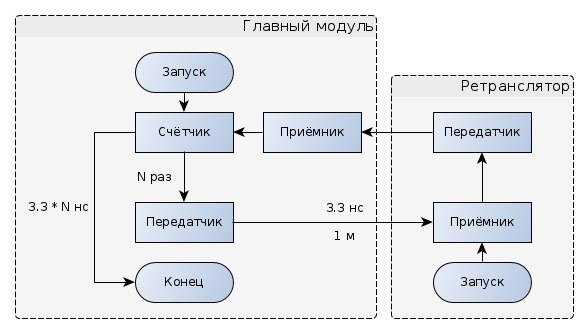
\includegraphics[width=1\linewidth]{Figures/accscheme.png}
    \caption{Функциональная схема метода <<накопления>> ToF}
    \label{fig:accscheme}
\end{figure}

Однако у данного метода есть и недостатки: чем ниже частота, тем больше будет время накопления результата. Для примера, возьмём частоту 1 Гц и расстояние 1 м. Тогда передатчик будет посылать данные приёмнику, ждать возврата сообщения, затем ждать секунду и посылать очередной пакет приёмнику.

На расстоянии 1 м. время полёта пакета от источника к приёмнику будет равно $T_f = \frac{1}{300.000.000} = 3.3$ нс.

Как будет сказано ниже, разрешение (погрешность) микроконтроллеров ATmega (Arduino) составляет около 4-10 мксек. В данном примере, возьмём 50 мксек для надёжности. Время, необходимое для того, чтобы микроконтроллер зарегистрировал изменение, будет равно:

\begin{equation}
t_w = \frac{\Delta\tau}{T_f} = \frac{50 \cdot 10^{-6}~\textrm{с}}{3.3 \cdot 10^{-9}~\textrm{с}} = 15151~\textrm{с} = 252~\textrm{мин} = 4.2~\textrm{ч}
\end{equation}

Обычно на практике применяются расстояния больше 1 метра, что сокращает время ожидания результата пропорционально расстоянию. Задача сводится к увеличению частоты работы устройства.
